\documentclass{report}
\usepackage{setspace}
%\usepackage{subfigure}

\pagestyle{plain}
\usepackage{amssymb,graphicx,color}
\usepackage{amsfonts}
\usepackage{latexsym}
\usepackage{a4wide}
\usepackage{amsmath}

\newtheorem{theorem}{THEOREM}
\newtheorem{lemma}[theorem]{LEMMA}
\newtheorem{corollary}[theorem]{COROLLARY}
\newtheorem{proposition}[theorem]{PROPOSITION}
\newtheorem{remark}[theorem]{REMARK}
\newtheorem{definition}[theorem]{DEFINITION}
\newtheorem{fact}[theorem]{FACT}

\newtheorem{problem}[theorem]{PROBLEM}
\newtheorem{exercise}[theorem]{EXERCISE}
\def \set#1{\{#1\} }

\newenvironment{proof}{
PROOF:
\begin{quotation}}{
$\Box$ \end{quotation}}



\newcommand{\nats}{\mbox{\( \mathbb N \)}}
\newcommand{\rat}{\mbox{\(\mathbb Q\)}}
\newcommand{\rats}{\mbox{\(\mathbb Q\)}}
\newcommand{\reals}{\mbox{\(\mathbb R\)}}
\newcommand{\ints}{\mbox{\(\mathbb Z\)}}

%%%%%%%%%%%%%%%%%%%%%%%%%%


\title{{\vspace{-14em} 
\includegraphics[scale=0.4]{ucl_logo.png}}\\
{{\Huge Project Title}}\\
{\large Optional Subtitle}\\
}
\date{Submission date: Day Month Year}
\author{Your name\thanks{
{\bf Disclaimer:}
This report is submitted as part requirement for the MY DEGREE at UCL. It is
substantially the result of my own work except where explicitly indicated in the text.
\emph{Either:} The report may be freely copied and distributed provided the source is explicitly acknowledged
\newline  %% \\ messes it up
\emph{Or:}\newline
The report will be distributed to the internal and external examiners, but thereafter may not be copied or distributed except with permission from the author.}
\\ \\
Name of your degree\\ \\
Supervisor's name}



\begin{document}
 
\onehalfspacing
\maketitle
\begin{abstract}
Summarise your report concisely.
\end{abstract}
\tableofcontents
\setcounter{page}{1}


\chapter{Title of first chapter}
This is just a bare minimum to get started.  There is unlimited guidance on using latex, e.g., {\tt https://en.wikibooks.org/wiki/LaTeX}.   You are still responsible to check the detailed requirements of a project, including formatting instructions, see \\
{\tt https://moodle.ucl.ac.uk/pluginfile.php/3591429/mod\_resource/content/7/UGProjects2017.pdf}.
Leave at least a line of white space when you want to start a new paragraph.

\section{Section 1}
Chapters should contain numbered sections and sub-sections.

\subsection{Sub-Section 1}
Remember that this is a structured technical/academic report, not an essay.

\section{Mathematical Notation}
Mathematical expressions are placed inline between dollar signs, e.g. $\sqrt 2, \sum_{i=0}^nf(i)$, or in display mode
\[ e^{i\pi}=-1\] and another way, this time with labels,
\begin{align}
\label{line1} A=B\wedge B=C&\rightarrow A=C\\
&\rightarrow C=A\\
\intertext{note that}
n!&=\prod_{1\leq i\leq n}i \\
\int_{x=1}^y \frac 1 x \mathrm{d}x&=\log y
\end{align}
We can refer to labels like this \eqref{line1}.   

\chapter{Title of second chapter}

The main chapters should start with a brief summary -- this chapter is about, or introduces, some aspect of the work.

\section{Main Content}
Often lots of citations here (and elsewhere), e.g. \cite{Rey:D} or \cite[Theorem 2.3]{PriorNOP70}.   Bibtex can help with this, but is not essential. If you want pictures, try

\begin{center}
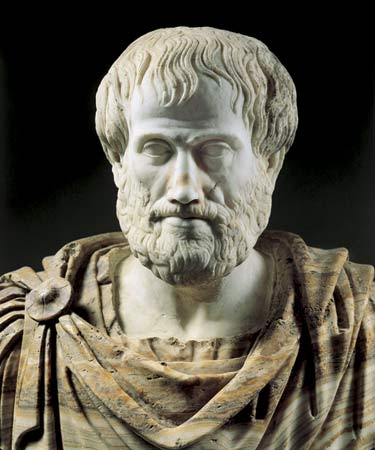
\includegraphics[scale=.5]{aristotle.jpg}
\end{center}
You can use 
\begin{itemize}
\item lists
\item like this
\end{itemize}
or numbered
\begin{enumerate}
\item like this,
\item or this
\end{enumerate}
but don't overdo it.

\section{More Content}

\section{Summary}
The main chapters should have a short summary, highlighting what the chapter has covered and any key points that need emphasising.

\chapter{Title of third chapter}
If you have a formal theorem you might try this.
\begin{definition}\label{def}
See definition~\ref{def}.
\end{definition}
\begin{theorem}
For all $n\in\nats,\; 1^n=1$.
\end{theorem}
\begin{proof}
By induction over $n$.
\end{proof}

\chapter{etc.}


\chapter{Conclusions}
\section{Achievements}
Summarise the achievements to confirm the project goals have been met.
\section{Evaluation}
Evaluation of the work (this may be in a separate chapter if there is substantial evaluation).

\section{Future Work}
How the project might be continued, but don't give the impression you ran out of time!

\appendix


\begin{thebibliography}{HHM99}


\bibitem[Pri70]{PriorNOP70}  %%only an example
A.~Prior.
\newblock The notion of the present.
\newblock {\em Studium Generale}, 23:  245--248, 1970.


\bibitem[Rey97]{Rey:D}
M.~Reynolds.
\newblock A decidable temporal logic of parallelism.
\newblock {\em Notre Dame Journal of Formal Logic}, 38(3):  419--436,
  1997.
\end{thebibliography}
\chapter{Other appendices, e.g., code listing}
Put your appendix sections here

\end{document}